\documentclass[12pt,a4paper]{article}
\usepackage[UTF8]{ctex}
\usepackage{amsmath,amssymb}
\usepackage{listings}
\usepackage{xcolor}
\usepackage{hyperref}
\usepackage{geometry}
\usepackage{graphicx}
\geometry{margin=2.5cm}

\lstdefinestyle{python}{
  language=Python,
  basicstyle=\ttfamily\small,
  keywordstyle=\color{blue}\bfseries,
  commentstyle=\color{gray},
  stringstyle=\color{red},
  showstringspaces=false,
  breaklines=true,
  frame=single,
  backgroundcolor=\color{gray!10}
}

\title{Bernstein-Vazirani Algorithm / Bernstein-Vazirani 算法}
\author{QuoNic}
\date{}

\begin{document}
\maketitle

\begin{center}
\textbf{Algorithms / 算法} | 难度：中级 | 预计时间：10 分钟
\end{center}

\tableofcontents
\newpage

%% ============================================================
\section{为什么需要？}

Bernstein-Vazirani 算法是 Deutsch-Jozsa 算法的推广，用于寻找隐藏的比特串。

\subsection{经典局限}
\b\begin{itemize}
  \item 经典算法需要 $n$ 次查询才能找到隐藏的比特串
  \item 每次查询只能获得 1 比特信息
\end{itemize}

\subsection{量子优势}
\b\begin{itemize}
  \item Bernstein-Vazirani 只需要 1 次查询
  \item 提供线性加速
  \item 是量子算法设计的范例
\end{itemize}

\subsection{实际应用}
\b\begin{itemize}
  \item 量子算法教学
  \item 量子优势验证
  \item 量子计算理论
\end{itemize}

%% ============================================================
\section{快速上手}

\begin{lstlisting}[style=python]
from quonic.algorithms import bernstein_vazirani

# Find hidden bit string
result = bernstein_vazirani("101", n_qubits=3)
print(f"Hidden string: {result.hidden_string}")
\end{lstlisting}

\textbf{预期输出}：
\begin{verbatim}
Hidden string: 101
\end{verbatim}

%% ============================================================
\section{原理详解}

\subsection{电路图}

\begin{center}
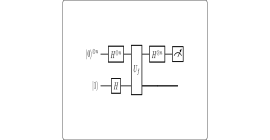
\includegraphics[width=0.6\textwidth]{../../images/bernstein_vazirani_circuit.svg}
\end{center}

\subsection{数学推导}

Bernstein-Vazirani 算法寻找隐藏的比特串 $s$，使得 $f(x) = s \cdot x \mod 2$。

\textbf{Step 1: 初始化}
\begin{equation}
|\psi_0\rangle = |0\rangle^{\otimes n}|1\rangle
\end{equation}

\textbf{Step 2: Hadamard 门}
\begin{equation}
|\psi_1\rangle = \frac{1}{\sqrt{2^n}} \sum_{x=0}^{2^n-1} |x\rangle \cdot \frac{|0\rangle - |1\rangle}{\sqrt{2}}
\end{equation}

\textbf{Step 3: Oracle 查询}
\begin{equation}
|\psi_2\rangle = \frac{1}{\sqrt{2^n}} \sum_{x=0}^{2^n-1} (-1)^{s \cdot x} |x\rangle \cdot \frac{|0\rangle - |1\rangle}{\sqrt{2}}
\end{equation}

\textbf{Step 4: Hadamard 门和测量}

测量结果就是隐藏的比特串 $s$。

\subsection{几何解释}

Bernstein-Vazirani 算法利用量子叠加态同时查询所有输入，通过干涉效应提取隐藏的比特串。

%% ============================================================
\section{代码详解}

\begin{lstlisting}[style=python]
from quonic.algorithms import bernstein_vazirani

# bernstein_vazirani(hidden_string, n_qubits)
# hidden_string: the hidden bit string to find
# n_qubits: number of qubits
result = bernstein_vazirani("101", n_qubits=3)

# result.hidden_string: the found hidden string
print(f"Hidden string: {result.hidden_string}")
\end{lstlisting}

%% ============================================================
\section{进阶用法}

\subsection{场景 1：不同隐藏串}

\begin{lstlisting}[style=python]
# Find different hidden strings
result = bernstein_vazirani("110", n_qubits=3)
print(f"Hidden string: {result.hidden_string}")
# Output: 110
\end{lstlisting}

\subsection{场景 2：多量子比特}

\begin{lstlisting}[style=python]
# More qubits for longer strings
result = bernstein_vazirani("10110", n_qubits=5)
print(f"Hidden string: {result.hidden_string}")
# Output: 10110
\end{lstlisting}

%% ============================================================
\section{适用场景}

\subsection{量子算法教学}

Bernstein-Vazirani 是量子算法的经典入门案例。

\subsection{量子优势验证}

Bernstein-Vazirani 是证明量子计算优势的算法之一。

\subsection{量子计算理论}

Bernstein-Vazirani 是量子算法设计的范例。

%% ============================================================
\section{常见问题}

\subsection{Bernstein-Vazirani 算法的加速比是多少？}

线性加速：经典需要 $n$ 次查询，量子只需要 1 次。

\subsection{Bernstein-Vazirani 算法有什么实际应用？}

Bernstein-Vazirani 主要用于教学和理论研究，实际应用有限。

\subsection{Bernstein-Vazirani 算法和 Deutsch-Jozsa 有什么区别？}

Deutsch-Jozsa 判断函数类型，Bernstein-Vazirani 寻找隐藏的比特串。

%% ============================================================
\section{学习路径}

\subsection{前置知识}
\b\begin{itemize}
  \item Deutsch-Jozsa 算法
  \item 量子比特和叠加态
  \item Hadamard 门和 CNOT 门
\end{itemize}

\subsection{继续学习}
\b\begin{itemize}
  \item Simon 算法
  \item Shor 算法
  \item 量子算法设计
\end{itemize}

%% ============================================================
\section{完整示例代码}

\subsection{示例 1：基本 Bernstein-Vazirani}

\begin{lstlisting}[style=python]
from quonic.algorithms import bernstein_vazirani

result = bernstein_vazirani("101", n_qubits=3)
print(f"Hidden string: {result.hidden_string}")
\end{lstlisting}

\

\section{下载}

\begin{itemize}
  \item [bernstein_vazirani.py](https://github.com/ChrisLee0721/QuoNic/blob/main/examples/bernstein_vazirani/bernstein_vazirani.py)
\end{itemize}

\end{document}
